\section{From Informational Agency to Operational Authority}
\subsection{Capability and authority are separate axes}
We define clinical agency as the capacity to choose and perform steps toward a healthcare task while interacting with an environment. Operational authority is permission, grounded in institutional context, to produce specified effects. A system can have extensive reasoning and tool capability but no permission to write clinical state. Conversely, a narrow automation can have permission to perform one operation without general reasoning. Figure~\ref{fig:agency} separates these dimensions.

A deployment description should identify what the agent can observe, propose, and commit; what a human must approve; and how completion is verified. ``Autonomous'' without these boundaries is insufficient. Local hosting governs infrastructure and data access, but cannot establish whether a clinical action is appropriate. Multi-agent debate can alter the reasoning process, but does not create institutional permission or independent clinical judgment.

\begin{figure}[t]\centering
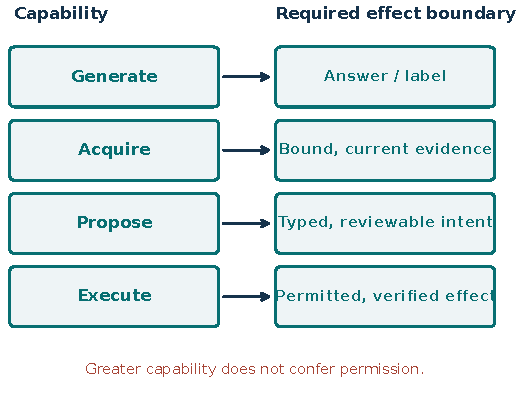
\includegraphics[width=\columnwidth]{figures/fig1_agency_authority.pdf}
\caption{Agency and authority are distinct. Each increased capability requires an explicit effect boundary and corresponding evidence; position does not imply clinical readiness.}\label{fig:agency}
\end{figure}

\begin{table}[t]\caption{Observable action classes and required distinctions}\label{tab:actions}\centering\footnotesize
\begin{tabularx}{\columnwidth}{@{}p{.23\columnwidth}YY@{}}\toprule
Class & Observable object & Essential distinction \\ \midrule
Informational answer & Text or label & Answer accuracy versus clinical effect.\\
Evidence acquisition & Retrieved observation & Availability versus freshness and patient binding.\\
Structured proposal & Typed operation & Plausible intent versus authorized commitment.\\
Sandbox commitment & Verified test-state change & Execution success versus real care.\\
Live bounded commitment & Destination receipt and state & Authorization versus clinical appropriateness.\\
Longitudinal delegation & Effects over time & Single action versus monitoring, omission, and recovery.\\ \bottomrule
\end{tabularx}\end{table}

\subsection{A trajectory is more than its final output}
For a task episode, let
\begin{equation}
\tau=\{(o_t,a_t,r_t,s_{t+1})\}_{t=1}^{T},
\end{equation}
where $o_t$ is an observation, $a_t$ a proposed or submitted action, $r_t$ a tool or destination receipt, and $s_{t+1}$ the subsequent state. The agent generally sees only part of the true clinical and technical state. A successful tool response may mean that a request was accepted, not that the intended effect occurred. A generated summary can claim completion despite an empty or incorrect destination result. Evaluators must therefore specify the state predicate that counts as success, how it is observed, and when that observation expires.

A write to a sandbox chart and a write to a live clinical record may use the same interface, yet have different authority and consequences. Table~\ref{tab:actions} distinguishes them. This taxonomy also separates research artifacts, such as executable analysis code, from clinical operations such as ordering a test. The former can be verified against software tasks without implying the latter are suitable for unsupervised use.

\subsection{Architecture does not determine evidence strength}
Single-agent loops, planner--executor arrangements, specialist panels, and multi-agent critics represent useful design options. Evidence should attach to a fully specified configuration: model/version, prompts, memory, retrieval corpus, tools, permissions, stopping rules, and budgets. Feedback memory may improve performance on a repeated task distribution while also changing the system being evaluated. Retrieval can ground answers in supplied material while exposing the planner to misleading or adversarial instructions. More components can add opportunities for cross-checking and also create correlated failure, inconsistent state, and communication overhead. The appropriate comparator is a matched workflow, not an architectural label.
